% =================================================================================================
\chapter{Biološke osnove} % Main chapter title
\label{bioloskeosnove} % For referencing the chapter elsewhere, use \ref{Chapter1} 
% =================================================================================================

U ovoj sekciji biće ukratko predstavljene biološke osnove neophodne za razumevanje rada i motivacije koja stoji iza određenih njegovih elemenata.
Najpre, biće opisano šta su proteini, koje su njihove osnovne funkcije i kakva im je struktura, a zatim će posebno biti opisani neuređeni proteini, njihova uloga i uzroci koji mogu dovesti do njihove pojave. 

% -------------------------------------------------------------------------------------------------
\section{Proteini}
\label{sec:proteini}
% -------------------------------------------------------------------------------------------------

Proteini (grč.~{\em protos} - $"$zauzimam prvo mesto$"$) su biološki makromolekuli, koji čine 70\% suve materije ćelija i  neophodni su za njihovu izgradnju i pravilno funkcionisanje. Osim uloge u izgradnji ćelija, učestvuju u mnogobrojnim procesima koji se odvijaju unutar organizma. Predstavljaju najvažniji sastojak žive materije i utiču na brojnost i raznolikost živih bića. Specifičnost proteina je tolika da svaka biljna i životinjska vrsta ima svoje proteine, dok se, kod viših organizama, razlikovanje može uočiti i na individualnom nivou. Broj proteina koji nastaju u živim bićima je ogroman, na primer $E. coli$ sa $3000$ i čoveka sa $5$ miliona proteina~\cite{spasic, Principi}.\\

Proteini su jedinjenja sačinjena od aminokiselina. Na osnovu broja aminokiselina koji ih čine peptidi, koji predstavljaju kraće nizove aminokiselina u odnosu na proteine, dele se na:
\begin{itemize}
\item oligopeptide - sastoje se od 10 ili manje aminokiselina, među njih spadaju dipeptidi, tripeptidi, itd. i 
\item polipeptide - sastoje se od 100 ili manje aminokiselina.
\end{itemize}

Proteini se mogu posmatrati i kao nizovi nadovezanih polipeptida.
Proteini i peptidi su izgrađeni od $22$ aminokiseline \footnote{Neki proteini u svom sastavu mogu da imaju $22$ različite aminokiseline. Pored $20$ standardnih aminokiselina (koji grade prirodne proteine), postoje i $2$ nestandardne i to su Selenocistein (eng.~{\em Selenocysteine}, simboli $Sec$, $U$) i Pirolizin (eng.~{\em Pyrrolysine},
simboli $Pyl$, $O$). Ove dve aminokiseline se ređe javljaju~\cite{MarijaJ}.}
Sve proteinske aminokiseline su $\alpha$-aminokiseline. Njih karakteriše to da su primarna amino i karboksilna grupa vezne za $\alpha$-ugljenikov atom. Aminokiseline se međusobno razlikuju po strukturi bočnog $R$-ostatka, koji utiče na strukturu proteina. Opšta strukturna formula aminokiselina može se videti na slici \ref{fig:aminokiselina}. % Principi  
\begin{figure}[h]
	\centering
    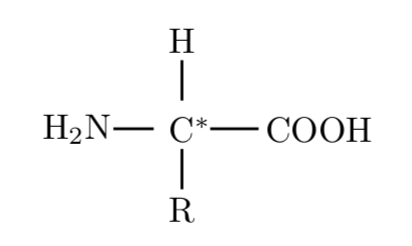
\includegraphics[width=0.5\textwidth]{Figures/BO/aminokiselina.png}
    \caption{Opšta strukturna formula aminokiselina ~\cite{Principi}}
    \label{fig:aminokiselina}
\end{figure}
Proteinske aminokiseline (osim glicina) imaju asimetričan $\alpha$-ugnjenikov atom i shodno tome mogu da se jave u dva oblika (prema Fišerovoj konvenciji) $L$ i $D$. Sve standardne aminokiseline imaju $L$-konfiguraciju. Grafički prikaz može se videti na slici \ref{fig:LDkonfig}.
\begin{figure}[H]
	\centering
    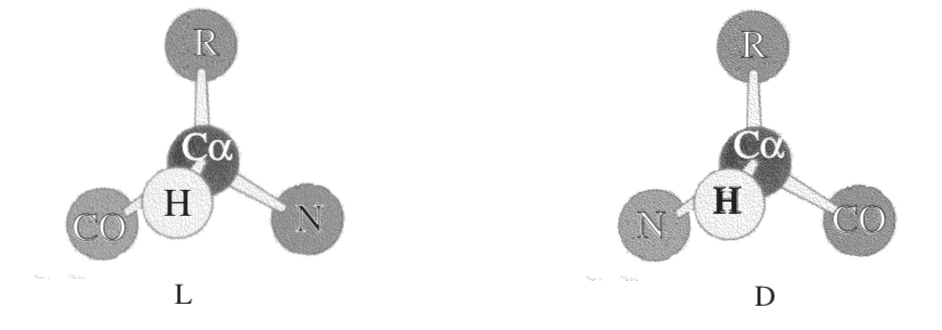
\includegraphics[width=0.5\textwidth]{Figures/BO/LDkonfig.png}
    \caption{Prikaz $L$ i $D$ prostorne konfiguracije ~\cite{Principi}}
    \label{fig:LDkonfig}
\end{figure}
U prirodi se pojavljuju $L-aminokiseline$ \footnote{$L-aminokiseline$ su one aminokiseline sa levom prostornom konfiguracijom, analogno, postoje i $D-aminokiseline$, sa desnom} i međusobno su povezane peptidnim vezama. Peptidne veze nastaju između $\alpha$-karboksilne grupe jedne aminokiseline i $\alpha$-amino grupe druge aminokiseline, pri čemu se oslobađa molekul vode (što je grafički prikazano na slici \ref{fig:peptidebonds}). Ovim postupkom nastaje nerazgranati polipeptidni lanac koji se sastoji od polipeptidne kičme i bočnih ostataka. Standardna grupa aminokiselina se može podeliti na esencijalne i
neesencijalne, čiji spisak se može videti u tabeli \ref{table:1}~\cite{MarijaJ,biopathways}.\\ 

\begin{figure}[H]
	\centering
    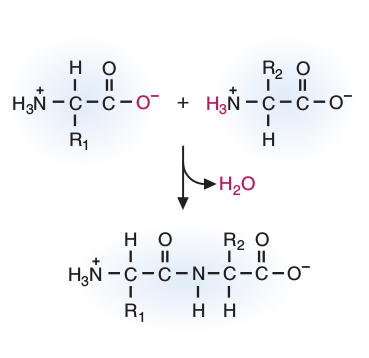
\includegraphics[width=0.5\textwidth]{Figures/BO/peptide_bonds.png}
    \caption{Prikaz spajanja $\alpha$-karboksilne grupe jedne aminokiseline i $\alpha$-amino grupe druge aminokiseline, pri čemu se oslobađa molekul vode ~\cite{bmbg}}
    \label{fig:peptidebonds}
\end{figure}

\begin{table}[h!]
\centering
	\begin{tabular}{|c c|} 
	\hline 
	Esencijalne & Neesencijalne \\ [0.5ex] 
	\hline\hline
	Arginin & Alanin \\ 
	\hline
	Histidin & Asparagin \\
	\hline
	Leucin & Asparaginska kiselina\\
	\hline
	Izoleucin & Cistein \\
	\hline
	Lizin & Glutaminska kiselina \\ [1ex] 
	\hline
	Metionin & Glutamin \\ [1ex] 
	\hline
	Fenilalanin & Glicin \\ [1ex] 
	\hline
	Treonin & Prolin \\ [1ex] 
	\hline
	Triptofan & Serin \\ [1ex] 
	\hline
	Valin & Tirozin \\ [1ex] 
	\hline
	\end{tabular}
\caption{Spisak esencijalnih i neesencijalnih aminokiselina}
\label{table:1}
\end{table}

Svaki molekul proteina nastaje u ćeliji živog organizma. Redosled aminokiselina u proteinskoj sekvenci određen je redosledom aminokiselina u dezoksiribonukleinskoj kiselini (DNK), odnosno gena, koji predstavljaju trojke nukleotida. Svakoj takvoj trojci jedinstveno je pridružena po jedna aminokiselina na osnovu genetskog koda. Proces kojim se enkodirana informacija prevodi iz DNK u niz aminokiselina u proteinskom lancu, posredstvom glasničke (eng.~{\em messenger}) ribonukleinske kiseline (RNK) i transportne (eng.~{\em transfer}) RNK, naziva se genska ekspresija. Proces sinteze proteina predstavlja \textit{centralnu dogmu molekularne biologije}, čiji se prikaz može videti na slici \ref{fig:dogma}~\cite{JKd}.

\begin{figure}[H]
	\centering
    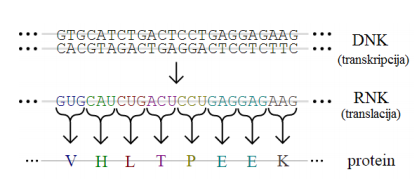
\includegraphics[width=0.5\textwidth]{Figures/BO/dogma.png}
    \caption{Prikaz centralne dogme molekularne biologije~\cite{JKd}}
    \label{fig:dogma}
\end{figure}

Pri deobi ćelije dolazi do replikacije DNK, čime je obezbeđeno da ćelija nove generacije primi ceo skup informacija neophodnih za njeno normalno funkcionisanje i razvoj. U procesu replikacije može doći do greške, odnosno mutacije, a kao posledica toga javljaju se dva problema:
\begin{itemize}
\item novonastala greška se prenosi na sve buduće generacije
\item  mutacija u genu proteina dovodi do izmena na aminokiselinskoj sekvenci što može dovesti do smrti ćelije. Vrlo retko se dešava da mutacija dovodi do poboljšanja, ali kada se to desi najčešće se to dešava na nivou populacije, čime se prirodnom selekcijom $"$stari$"$ gen menja u potpunosti  ~\citep{Principi}.
\end{itemize}


\subsection{Funkcije i osobine proteina}
%~\cite{JKd}
Pri istraživanju bioloških procesa neophodno je znati i dobro razumeti funkcije proteina. To se posebno može uočiti kod proučavanja oboljenja ljudi, ako se u obzir uzme činjenica da se mnoga oboljenja pojavljuju kao posledica funkcionalnih mutacija. Proteini su biološki najaktivniji molekuli sa velikim brojem esencijalnih funkcija koje se dele na:
\begin{itemize}
\item \textit{dinamičke}, od kojih su najvažnije:
\begin{enumerate} 
\item transportna - prenos molekula (poput kiseonika, gvožđa, lipida) i hormona od mesta sinteze do mesta delovanja,
\item biološka - regulacija metaboličkih procesa u ćeliji, kontrola i regulacija transkripcije gena i translacija,
\item katalizatorska - biološka katalizacija \footnote{Katalizacija predstavlja proces povećavanja brzina reakcija},
\item zaštitna - keratin, koagulacija krvi,
\item održavanje zapremine tečnosti u organizmu,
\end{enumerate}
\item \textit{strukturne}, od kojih su najvažnije:
\begin{enumerate}
\item obezbeđivanje čvrstine i elastičnosti organa,
\item davanje oblika organizmu,
\item izgradnja strukturnih elemenata ćelije i
\item bitna uloga u kontraktilnim i pokretnim elementima organizma.
\end{enumerate}
\end{itemize} 
U tabeli \ref{table:4} mogu se videti primeri nekih proteina i njihovih uloga.

\begin{table}[H]
\centering
 \begin{tabular}{|c | @{\extracolsep{\fill}}c|} 
 \hline
Naziv proteina & Aktivnost/Funkcija/Nalaženje\\ [0.5ex] 
 \hline\hline
 Enzimi & Kataliza svih reakcija u živim sistemima \\ 
 \hline
 Transportni proteini & \\
 Hemoglobin & transport kiseonika i ugljendioksida  \\ 
 Mioglobin & transport kiseonika u mišićima  \\ 
 Serum albumin & transport masnih kiselina, lekova,...  \\ 
 \hline
 Kontraktilni proteini & \\
 Miozin & pokretljivost mišića  \\ 
 Aktin &   \\ 
 \hline
 Zaštitni proteini & \\
 Imunoglobulini & stvaraju kompleks sa stranim telom  \\ 
 Fibrinogen & prekursor fibrina pri zgrušavanju krvi \\ 
 Trombin & komponenta u zgrušavanju krvi  \\ 
 \hline
  Hormoni & \\
 Insulin & reguliše metabolizam glukoze  \\ 
 Hormoni rasta &  stimulišu rast \\ 
 \hline
  Rezervni proteini & rezerva aminokiselina za mladu jedinku\\
 Ovalbumin & jaje  \\ 
 Kazein & mleko \\ 
 Gliadin & pšenica  \\ 
 \hline
  Strukturni proteini &\\
 $\alpha$-keratin & kosa, koža, krzno, nokti  \\ 
 Fibroin & svila, paukova mreža\\ 
 Kolagen & vezivno tkivo  \\ 
 \hline
\end{tabular}
\caption{Primeri proteina.~\cite{Principi}}
\label{table:4}
\end{table}

Neke od karakteristika proteina koje su bitne u kontekstu strukture su:
\begin{itemize}
\item proteini grade kompleksna jedinjenja sa različitim supstancama po principu strukturne komplementarnosti i  
\item proteini poseduju visoku osetljivost na različite agense koji ih denaturišu \footnote{Denaturacija proteina je proces koji izaziva promene u strukturi proteina, čime se menja i njihov fiziološki uticaj.}. Neki od najčešćih agenasa su: visoka temperatura, pritisak, mehaničko tretiranje, dejstvo kiselina, baza, organskih rastvarača, materija, itd.~\cite{spasic,JKd}.
\end{itemize}
 
\subsection{Struktura proteina}
Osnovna struktura proteinskog molekula sastoji se od polipeptidnog niza aminokiselina povezanih peptidnom vezom. \textit{Aminokiselinska} sekvenca je redosled kojim su povezane aminokiseline. Polipeptidni niz se spontano na različite načine uvija  u kompleksnu trodimenzionalnu strukturu, koja se smatra najstabilnijom. Struktura proteina zavisi od redosleda aminokiselina i utiče na njegovu funkciju. Unutrašnjost takve strukture ima visoku gustinu, pa polipeptidni lanac ne dopušta promene u sastavu i zahteva prisustvo aminokiselina tačno određene veličine. Uobičajena raspodela aminokiselina u proteinima je daleko od ravnomerne. Neke aminokiseline se javljaju mnogo češće od ostalih, na primer, leucin se pojavljuje devet puta više od triptofana
~\cite{spasic,Principi,biopathways}. \\

Proteinsku strukturu održavaju različite vrste kovalentnih i nekovalentnih interakcija između hemijskih jedinjenja, na primer: vodonične, jonske, elektrostatičke, dipolne, itd.. Nabiranjem i uvijanjem lanaca kreiraju se različiti oblici proteina: vlaknasti, globularni ili eliptični. Strukturni proteini su vlaknasti, dok su oni koji pokazuju određenu aktivnost globularni. Ako mutacija dovede do toga da aminokiselina sa malim bočnim lancem bude zamenjena aminokiselinom sa velikim, pojaviće se problem u formiranju trodimenzionalne strukture. Ako bi se, pak, velika aminokiselina zamenila sa malom, pojavio bi se prazan prostor, što bi moglo dovesti do destabilizacije molekula proteina~\cite{spasic,Principi,biopathways,medbio}. \\

Obično se struktura proteina posmatra u nivoima, pa tako postoji hijerarhijska strukturalna organizacija u četiri nivoa:
\begin{enumerate}
\item primarna,
\item sekundarna,
\item tercijarna i
\item kvaternarna.
\end{enumerate}
Na slici \ref{fig:structures} se može videti opšti prikaz mogućih struktura proteina, a na drugoj slici \ref{fig:structures2} šematski prikaz~\cite{spasic}.
\begin{figure}[H]
	\centering
    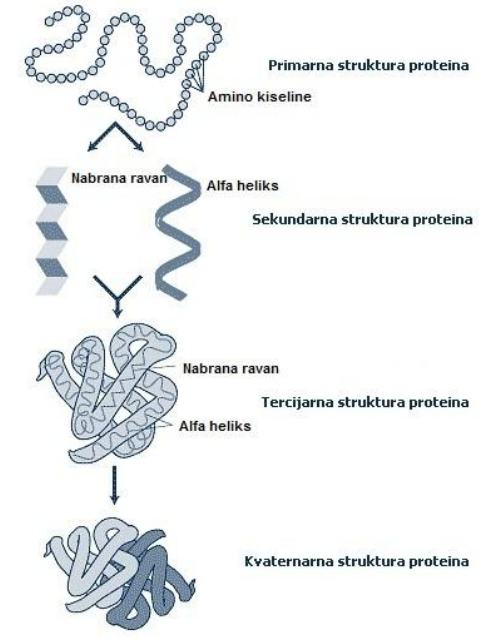
\includegraphics[width=0.5\textwidth]{Figures/BO/protein_structures.png}
    \caption{Prikaz struktura proteina \ref{wiki}}
    \label{fig:structures}
\end{figure}
\begin{figure}[H]
	\centering
    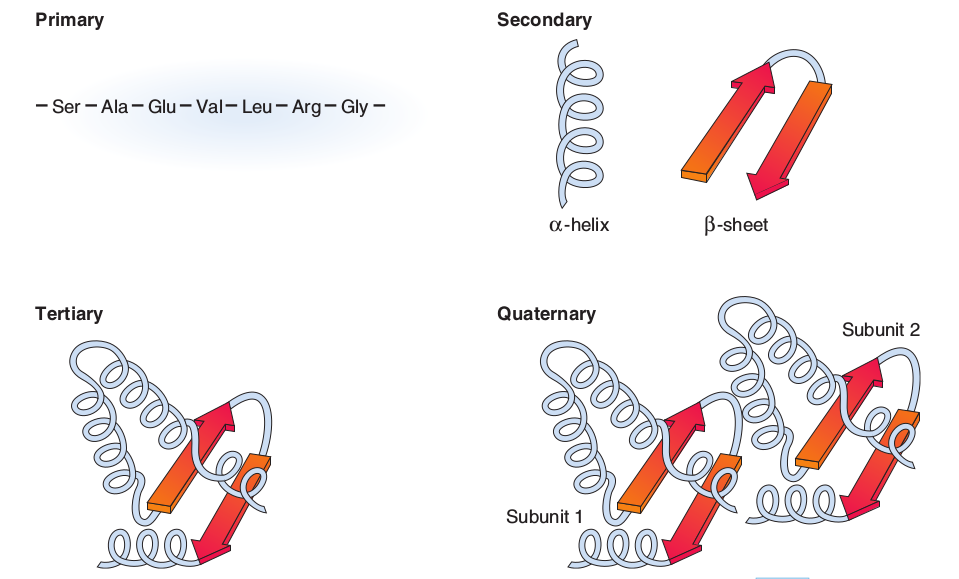
\includegraphics[width=1\textwidth]{Figures/BO/structure_schema.png}
    \caption{Šematski prikaz struktura proteina~\cite{bmbg}}
    \label{fig:structures2}
\end{figure}
Određivanje sastava proteina u vidu aminokiselina je relativno jednostavno, dok je određivanje odnosa između sastava aminokiselina i strukture proteina komplikovano. Uprkos tome, često se mogu izvući korisni zaključci o strukturi proteina na osnovu aminokiselinskog sastava~\cite{Principi}.

\subparagraph{Primarna struktura}
Predstavlja s\^amu sekvencu aminokiselina\footnote{Redosled kojim su aminokiseline poređane u nekom polipeptidu se zove sekvenca aminokiselina~\cite{spasic}.} koje učestvuju u izgradnji proteina. Ova struktura ima ključni značaj za određivanje funkcije proteina zbog interakcija koje se javljaju između bočnih lanaca aminokiselina, a koji utiču na trodimenzionalnu strukturu. Proteini koji poseduju sličnu sekvencu aminokiselina nazivaju se $homologi$, a poređenje sekvenci među takvim proteinima može ukazati na genetsku relaciju između različitih vrsta.Prikaz izgleda primarne strukture na primeru insulina kod čoveka se vidi na slici \ref{fig:insulin}~\cite{spasic}.\\
\begin{figure}[H]
	\centering
    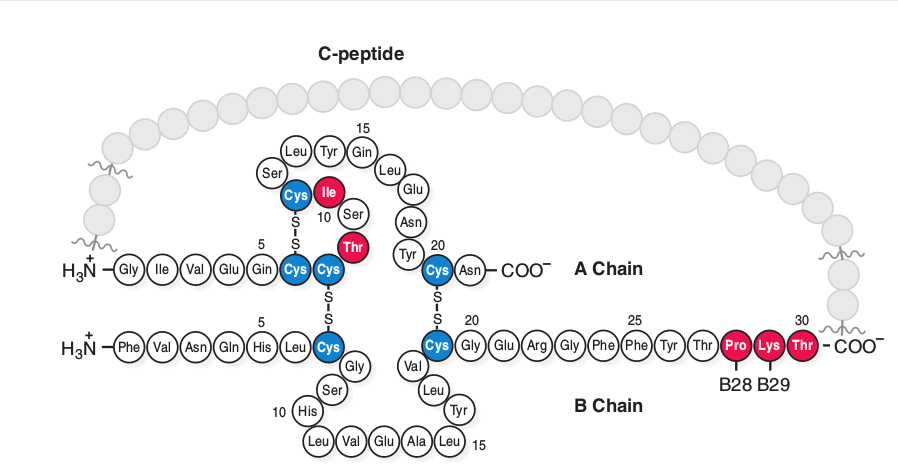
\includegraphics[width=1\textwidth]{Figures/BO/insulin.png}
    \caption{Prikaz primarne strukture~\cite{bmbg}}
    \label{fig:insulin}
\end{figure}

Mnoge genetske bolesti rezultuju u proteinima sa poremećenim redosledom aminokiselina, što uzrokuje nepravilno presavijanje i gubitak ili nemogućnost normalnog funkcionisanja. Ukoliko su nam poznate strukture normalnih i mutiranih proteina, te informacije možemo iskoristiti za dijagnostikovanje ili proučavanje bolesti. Promene u primarnoj strukturi mogu imati uticaja i na više nivoe proteinskih struktura. Takve promene često dovode do lošeg presavijanja proteina i mogu dovesti do njegovog gubitka funkcije~\cite{flash,lippincott}.

\subparagraph{Sekundarna struktura}
Odnosi se na oblik koji protein zauzima u prostoru i označava pravilno pojavljivanje ponavljanog prostornog rasporeda primarne strukture, u jednoj dimenziji. Ovu strukturu čini nekoliko različitih oblika, od kojih su najčešći $\alpha$-heliks i $\beta$-presavijena traka (ili $\beta$-struktura), a čest je i tzv. $\beta$-okret~\cite{spasic,medbio}.\\
\textbf{$\alpha$-heliks} je tip sekundarne strukture kod kog se gusto pakovani polipeptidni lanac spiralno uvrće. Karakteriše se brojem peptidnih jedinica po okretu i rastojanjem između dva okreta. Predstavlja najrasprostranjeniju sekundarnu strukturu i energetski je veoma siromašan iz čega se može zaključiti da je dosta stabilan. Javlja se kod globularnih i fibrilnih proteina. Heliks mogu obrazovati i $L-$ i $D-$ aminokiseline, pa postoje i dva tipa heliksa: levi i desni (u zavisnosti na koju stranu se navija, desni se navija u pravcu prstiju desne ruke kada se palac postavi u pravcu ose heliksa). Prikaz izgleda $\alpha$-heliksa se vidi na slici \ref{fig:aheliks}~\cite{spasic, Principi}.
\begin{figure}[H]
	\centering
    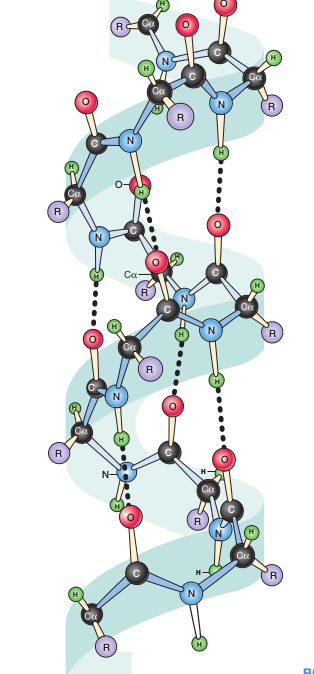
\includegraphics[width=0.25\textwidth]{Figures/BO/ahelix.png}
    \caption{Prikaz $\alpha$-heliksa~\cite{bmbg}}
    \label{fig:aheliks}
\end{figure}
\textbf{$\beta$-traka} za razliku od $\alpha$-heliksa se sastoji od dva ili više peptidnih lanaca, ili segmenata polipeptidnih lanaca, a obrazuje se kada se ovakvi tipovi lanca povežu uzdužno vodoničnim vezama. Razlika između polipeptidnog niza u  $\beta$-traci i potpuno istegnutog polipeptidnog niza je u tome što je kod  $\beta$-trake taj polipeptidni niz nabrane strukture. Postoje dva tipa $\beta$-traka: 
\begin{itemize}
\item paralelna - vodonično su vezani susedni polipeptidni nizovi istih smerova  i 
\item antiparalelna - vodonično su vezani susedni polipeptdni nizovi suprotnih smerova. 
\end{itemize}
Moguće su i mešovite paralelne-antiparalelne strukture.
$\beta$-trake se često javljaju u proteinima, a u globularnim proteinima se podjednako često javljaju i paralelne i antiparalelne. Sekundarna struktura se eksperimentalno utvrđuje na osnovu kristalne strukture proteina.
Prikaz izgleda $\beta$-trake se vidi na slici \ref{fig:beta}~\cite{spasic, Principi}.\\
%dodati mozda ovde primere proteina koji imaju sekundarnu strukturu
\begin{figure}[h]
	\centering
    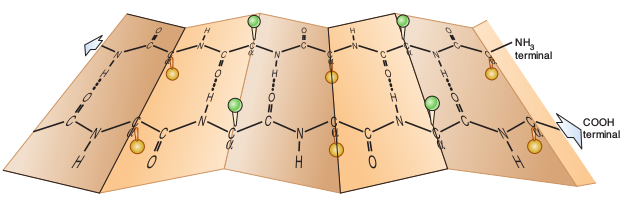
\includegraphics[width=1\textwidth]{Figures/BO/beta.png}
    \caption{Prikaz $\beta$-trake~\cite{bmbg}}
    \label{fig:beta}
\end{figure}
\textbf{$\beta$-okreti} - obrću pravac polipeptidnog lanca praveći kompaktan globularan oblik~\cite{lippincott}. 
 
Prikaz izgleda sekundarnih struktura se nalazi na slici \ref{fig:ab}.
\begin{figure}[h]
	\centering
    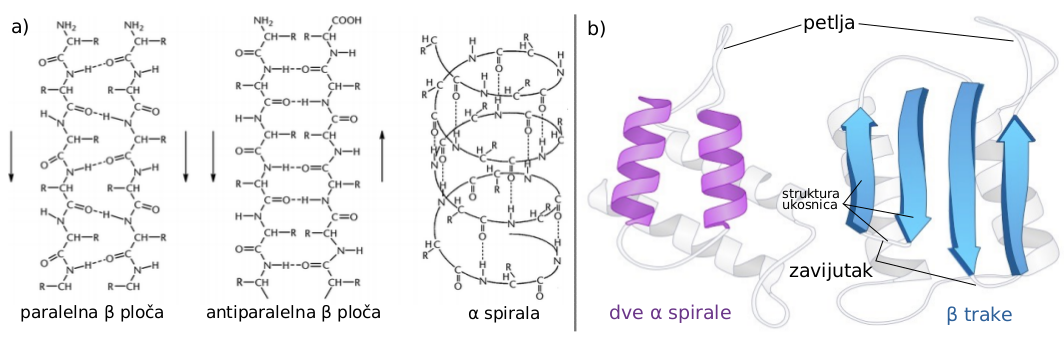
\includegraphics[width=1\textwidth]{Figures/BO/sec_structure.png}
    \caption{Prikaz sekundarnih struktura~\cite{Vinterhalter}}
    \label{fig:ab}
\end{figure}

\subparagraph{Tercijarna struktura}
Kod globularnih proteina se polipeptidni niz uvija u kompaktnu globulu. Tercijarna struktura proteina predstavlja unutarmolekularno slaganje polipeptidnog lanca u kompaktnu trodimenzionalnu strukturu specifičnog oblika (globule), koja nastaje prostornim organizovanjem polipeptidnog lanca, sa sekundarnom strukturom. Na taj način se približavaju ostaci aminokiselina koji su udaljeni u primarnoj strukturi. Tercijarna struktura predstavlja način organizacije, odnosno rasporeda, sekundarnih struktura i položaj bočnih ostataka aminokiselina. Proteini ove strukture su globularni i kompaktni sa velikom gustinom u središtu. Poznavanje ove strukture proteina predstavlja osnovu za izučavanje funkcije i aktivnosti proteina. Kako bi se eksperimentalno utvrdila ova struktura vrši se rendgenska strukturna analiza.~\cite{spasic, Principi,medbio}.

\subparagraph{Kvaternarna struktura}
Predstavlja agregaciju više peptidnih lanaca u molekulu proteina. Mnogi proteini, posebno oni velike mase, izgrađeni su od nekoliko polipeptidnih lanaca. Svaka takva komponenta naziva se $podjedinica$ ili $protomer$. Oni mogu biti identični\footnote{Tada takve proteine nazivamo $oligomerima$} ili se razlikovati prema strukturi. Ovakav raspored dovodi do brzog i efikasnog transfera supstrata od jednog aktivnog centra enzima do drugog. Prikaz proteina sa kvatenarnom strukturom može se videti na ~\ref{fig:hemoglobin} ~\cite{spasic,medbio}.
\begin{figure}[h]
	\centering
    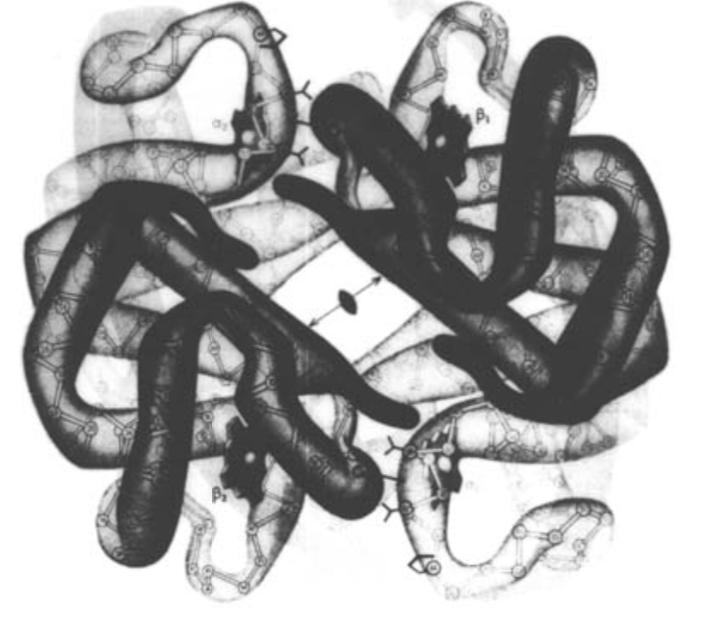
\includegraphics[width=0.5\textwidth]{Figures/BO/hemoglobin.png}
    \caption{Prikaz hemoglobina, predstavnika globularnih proteina sa kvatenarnom strukturom~\cite{Principi}}
    \label{fig:hemoglobin}
\end{figure}  
Postoji nekoliko razloga iz kojih se kvaternarna struktura javila:
\begin{itemize}
\item Kompleksnija uloga zahteva kompleksniju strukturu 
\item Veća efikasnost katalitičkih procesa - katalizacija niza reakcija u metaboličkom procesu vrši se enzimima spojenih u multienzimske komplekse
\item Viši nivo može da utiče na niži nivo strukture, pa tako kvaternarna struktura može da utiče na tercijarnu strukturu što se ogleda u njihovoj aktivnosti. Time se uvodi kooperativnost među subjedinicama. Posledica ovoga je regulacija i kontrola važnih biohemijskih procesa u ćeliji. 
\item Efikasnija biosinteza i lakše odstranjivanje grešaka pri procesu biosinteze.
\end{itemize}
 Da bismo mogli da izučavamo kvaternarnu strukturu neophodno je obratiti pažnju na nekoliko bitnih aspekata. Prvi se odnosi na \textit{stehiometriju}, odnosno, tip i broj podjedinica koje čine kvaternarnu strukturu. Drugi se odnosi na \textit{geometriju}, odnosno, raspored podjedinica geometrijski, kao i tipove simetrije. Treći aspekt je \textit{stabilnost kvaternarne strukture}. Stabilnost se odnosi na energetske aspekte interakcija i prirode kontakata između podjedinica. Naredni aspekt je \textit{funkcionalni}, odnosno kako komunikacija među podjedinicama utiče na biološku funkciju. Poslednji aspekt odnosi se na \textit{komunikaciju među podjedinicama} ~\cite{Principi}.
 
\subsection{Savijanje proteina}
Izučavanje uvijanja i razvijanja proteina doprinosi razumevanju nastanka određene strukture proteina. Interakcije između lanaca aminokiselina koji se nalaze sa strane, određuju kako se dugački polipeptidni lanac presavija u trodimenzionalni oblik funkcionalnog proteina. Presavijanje proteina koje se događa u ćeliji traje od nekoliko sekundi do nekoliko minuta. 
Na slici \ref{fig:folding} se može videti opšti prikaz savijanja proteina.
\begin{figure}[h]
	\centering
    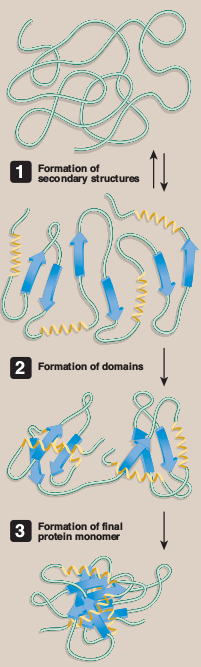
\includegraphics[width=0.25\textwidth]{Figures/BO/protein_folding.png}
    \caption{Prikaz savijanja proteina~\cite{lippincott}}
    \label{fig:folding}
\end{figure}


\subsection{Denaturacija proteina}
Denaturisanje proteina rezultuje u odvijanju i dezorganizaciji proteinske sekundarne i tercijarne strukture. U idealnim uslovima, denaturisanje proteina može biti $reverzibilno$. To znači da bi se protein, pri prestanku delovanja agenasa, vratio u normalno stanje. Međutim, većina proteina ostaje trajno neuređena. O neuređenosti proteina biće više reči u nastavku.\\

Jedno od objašnjenja zašto se protein ne vraća u originalno stanje se sastoji u tome da protein počinje sa savijanjem pre nego što se izvrši sinteza celog lanca. Osim toga, specijalizovana grupa pomoćnih proteina (engl. $chaperones$) je neophodna za pravilno savijanje mnogih vrsta proteina. Ovi pomoćni proteini interaguju sa polipeptidima u nekoliko faza tokom procesa savijanja, imaju ulogu u tome da održavaju protein nesavijenim dok sinteza nije gotova, ili imaju ulogu katalizatora. Loše savijanje proteina može dovesti do različitih bolesti kao što su amiloidna bolest ili Prionova bolest~\cite{lippincott}.

% -------------------------------------------------------------------------------------------------
\section{Neuređenost proteina}
% -------------------------------------------------------------------------------------------------

Eksperimentalnim utvrđivanjem sekundarne strukture proteina (koje će biti detaljnije opisano u \ref{eksperimentalno}) uočeno je da se neretko, pod određenim fiziološkim uslovima, javljaju proteini sa trodimenzionalnom strukturom koja nije dobro definisana.
Neuređenost predstavlja inherentno\footnote{Inherentno = nasleđeno} svojstvo sekvence. Neuređen može biti ceo protein, a mogu biti neuređeni određeni regioni proteina različitih dužina. Kao posledica, ovakve proteine nazivamo inherentno neuređenim proteinima, skraćeno IDP\footnote{eng.~{\em Intrinsically Disordered Proteins}}, a ako su u pitanju neuređeni, ali funkcionalni, regioni, onda je skraćenica IDPr\footnote{eng.~{\em Intrinsically Disordered Protein Regions}}. Strukturalni poremećaji su česti kod viših eukariota. Kod ljudi, čak trećina svih proteina ima neuređenu strukturu. Neuređeni proteini su uključeni u procese stvaranja mnogih bolesti poput raka, neurodegenerativnih i kardiovaskulatnih bolesti, dijabetesa, brojnih neuronskih oboljenja i drugih. Statističkom analizom došlo se do zaključka da se aminokiseline mogu klasterovati na dve grupe: 
\begin{enumerate}
\item aminokiseline koje promovišu uređenost (eng.~{\em order promoting}) i
\item aminokiseline koje promovišu neuređenost (eng.~{\em disorder promoting}).
\end{enumerate}
Neuređene proteine ili neuređene regione je teško kategorizovati, a jedan od opštih opisa strukture dat je kao kombinacija više tipova foldona\footnote{Foldon ostaje u originalnom nazivu, kao posledica manjka literature~\cite{Vinterhalter}.}:
\begin{itemize}
\item foldon (eng.~{\em foldon}) je nezavisno organizujuća jedinica(region) proteina,
\item indukativni foldon (eng.~{\em inducible foldon}) je neuređeni region proteina koji savijanje lanca postiže barem delom vezivajući se za partnera,
\item ne-foldon (eng.~{\em non-foldon}) je neuređeni region proteina koji nikada ne postiže uređenost,
\item polu-foldon (eng.~{\em semi-foldon}) je neuređeni region proteina koji ostaje polovično neuređen i nakon vezivanja za partnera, i 
\item anti-foldon (eng.~{\em unfoldon}) je region proteina koji iz uređenog prelazi u neuređeno stanje u cilju izvršavanja neke funkcije.
\end{itemize}

Postoji nekoliko mogućih stanja (oblika) u kojima se protein može naći. Ova stanja i prelazi između njih(neki proteini mogu prelaziti iz neuređenog u uređeno stanje, i obratno), prema {\em hipotezi proteinskog trojstva}, utiču na funkciju proteina. Svaki od mogućih oblika proteina može biti njegovo prirodno stanje i imati uticaja na njegovu ulogu u ćeliji. Proteini se mogu pojavljivati u raznim oblicima:
\begin{enumerate}
\item uređen protein,
\item topljiva globula (eng.~{\em molten globule}),
\item pre-topljiva globula (eng.~{\em pre-molten globule}) i 
\item nasumično klupko (eng.~{\em random coil}).
\end{enumerate}

Neuređenost proteina se utvrđuje eksperimentalno, laboratorijskim analizama, ili uz pomoć prediktora za automatsko utvrđivanje neuređenosti~\cite{JKd,IDP,IDPIDPr,DPC, IDPiH, BinaryClass}. 

\subsection{Eksperimentalno ispitivanje neuređenosti proteina}
\label{eksperimentalno}
Eksperimentalno utvrđivanje neuređenosti proteina podrazumeva laboratorijsko utvrđivanje neuređenosti korišćenjem raznih biofizičkih i biohemijskih tehnika i njihovih kombinacija. Eksperimentalno utvrđivanje neuređenosti je veoma skupo i nedovoljno brzo, zbog čega ne može da ispuni sve zahteve koje postavljaju akademija i industrija. Uprkos tome, razvijen je veliki broj metoda za karakterizaciju strukture i osobina proteina. Svaka eksperimentalna metoda karakteriše se raznim prednostima manama i nivoom pouzdanosti, zbog čega je najbolje kombinovati dobijene rezultate. Naredne eksperimentalne, biofizičke i biohemijske, tehnike su najčešće u ispitivanju neuređenosti proteina~\cite{JKd, IDP}:
\begin{itemize}
\item Kristalografija X-zracima(eng.~{\em X-ray crystallography}),
\item Spektroskopija nuklearnom magnetnom rezonancom (eng.~{\em NMR spectroscopy}),
\item Cirkularni dihroizam (eng.~{\em Circular dichroism (CD) spectroscopy}),
\item Osetljivost na proteolizu (eng.~{\em Sensitivity to proteolysis}),
\item Ramanova optička aktivnost, itd. 
\end{itemize}
Navedene metode neće biti detaljnije obrazlagane jer prevazilaze domene ovog rada. 

\subsection{Računarsko ispitivanje neuređenosti proteina}

Kao posledica osobina eksperimentalnog ispitivanja neuređenosti, veliki napori su uloženi u razvoj prediktora za računarsko utvrđivanje neuređenosti proteina. Ovi prediktori uz pomoć računara, korišćenjem tehnika mašinskog učenja, vrše utvrđivanje neuređenosti proteina. Iz godine u godinu, broj ovih prediktora je sve veći, a u poslednje vreme se radi i na kreiranju metaprediktora, koji predviđanje vrše kombinovanjem više tehnika. O ovoj vrsti predikcije biće više reči u narednom poglavlju.\\
